\paragraph{Apache Sling}
\label{sec:sling}\index{Apache Sling}
Ein weiterer Bestandteil von \ac{aem} ist Apache Sling. Dieses Framework zum Erstellen von serverseitigen Webanwendungen benötigt eine \ac{jcr}-Implementierung wie Apache Jackrabbit oder, wie im Fall von \ac{aem}, \ac{crx}. 
Anhand des angeforderten Pfades bei einem HTTP-Request wird entschieden, welches Skript bzw. Servlet ausgeführt werden soll und welche Daten aus dem \ac{jcr} benötigt werden. Ziel von Apache Sling ist es, Inhalte aus dem \ac{jcr} über ein HTTP-Request nach dem \ac{rest}\index{REST}-Programmierparadigma bereitzustellen. Für \ac{rest} müssen folgende Eigenschaften erfüllt werden \cite[S. 82 f.]{ste15}.		

\begin{itemize}
	\item Jede Web-Ressource ist über einen eindeutigen \ac{url} zu erreichen.
	\item Auf Web-Ressourcen können verschiedene Methoden angewandt werden. Bei \ac{http} wären dies z. B. POST, GET DELETE oder PUT. Zu beachten ist, dass \ac{rest} jedoch kein \ac{http} voraussetzt.
	\item Die Darstellung von Web-Ressourcen kann in verschiedenen Formaten erfolgen.
	\item \ac{rest} ist immer zustandslos.
\end{itemize}

\autoref{img:sling} beschreibt, wie Apache Sling einen Aufruf auflöst. 

\begin{figure}[H]
	\begin{center}
		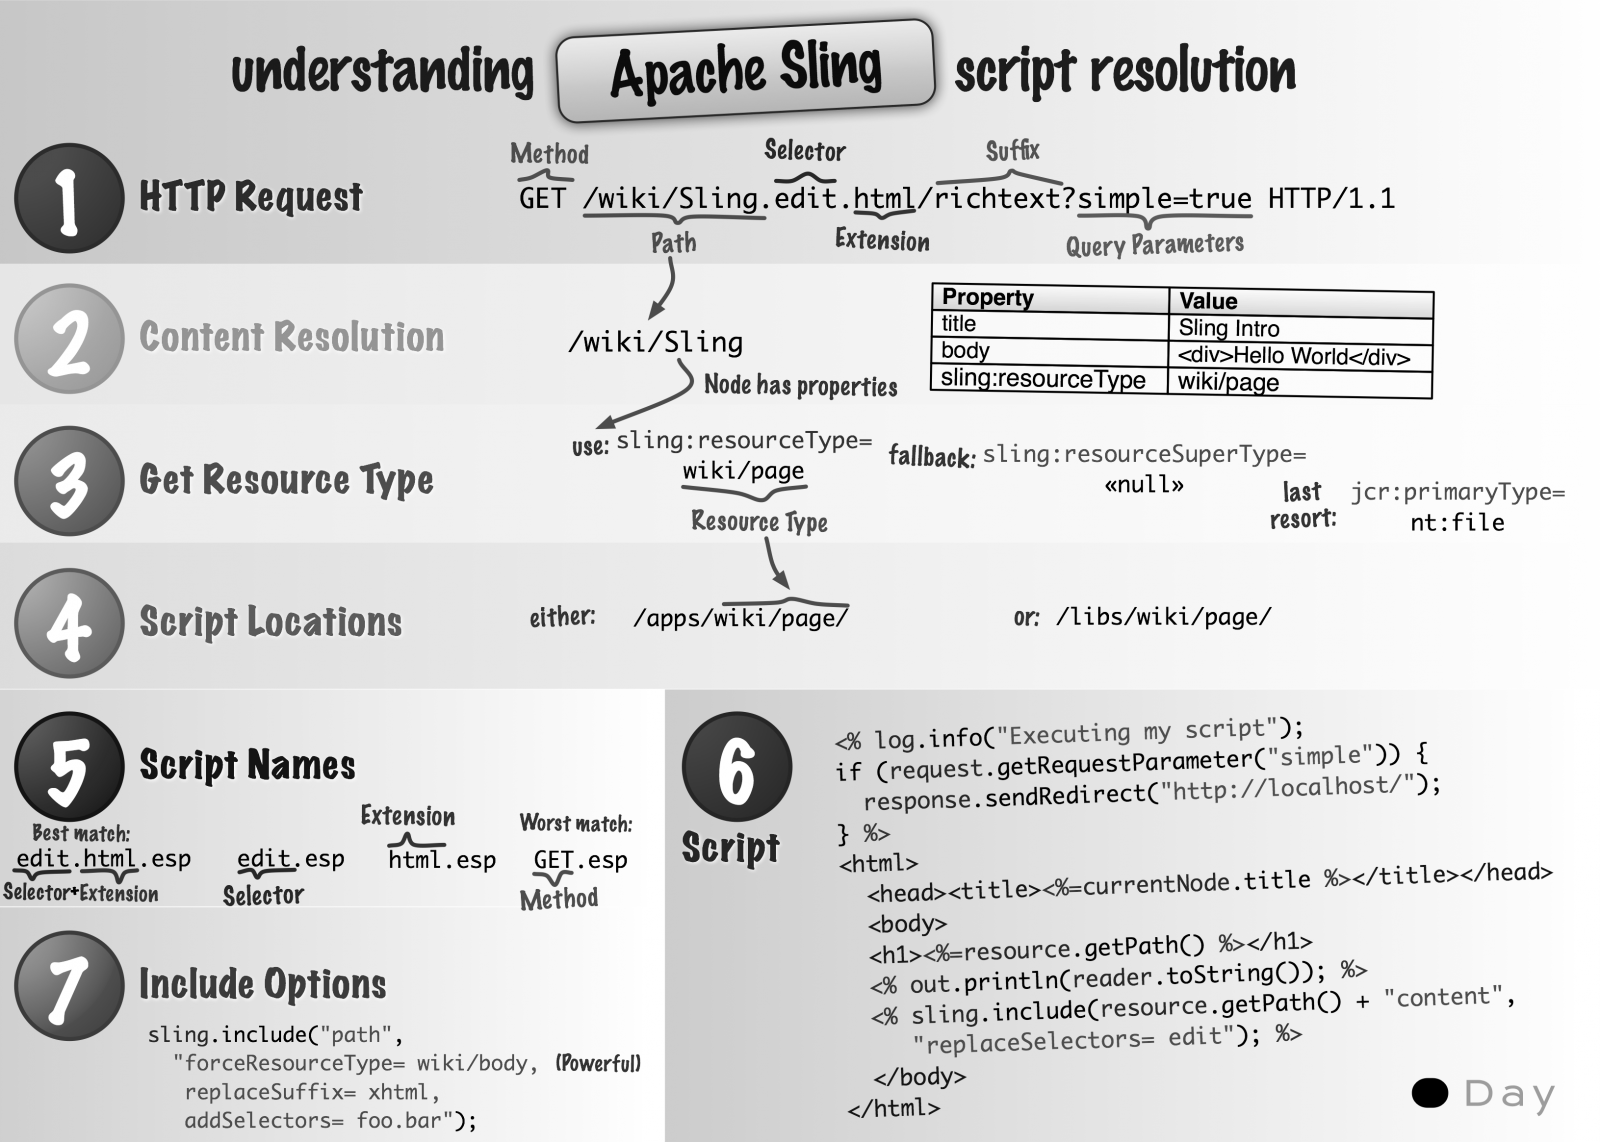
\includegraphics[width=1\textwidth]{sling_bw.png}
		\caption{Auflösung einer Anfrage bei unter Sling, von \cite{adobe_sling}}
		\label{img:sling}
	\end{center}
\end{figure}

Wird z. B. die Seite über einen Webbrowser \pseudourl{http://localhost:4502/wiki/Sling.edit.html/richtext?simple=true} aufgerufen, so wird die URL aufgeteilt. Alles ab \quotes{/wiki...} wird von Sling aufgelöst, somit wird im Folgenden nur der Abschnitt ab \quotes{/wiki...} betrachtet.
\begin{enumerate}
	\item Alles bis zum ersten Punkt ist der Pfad, gefolgt von einem oder mehreren Selektoren und zuletzt der Erweiterung. Anschließend können noch Suffixe und Parameter folgen, die noch weitere Informationen mitgeben.
	\item Die Eigenschaften des Knotens, die sich aus dem vorherigen Schritt erschlossen haben, werden abgefragt und nach einer mit dem Namen. \quotes{sling:resourceType} gesucht. Diese hat in diesem Beispiel den Wert \quotes{wiki/page}.
	\item Der Wert wird für den nächsten Schritt verwendet.
	\item Nun wird zunächst unter /app/wiki/page nach einem geeigneten Skript gesucht. Wird dieses nicht gefunden, wird die Suche unter /libs/wiki/page fortgesetzt.
	\item Der Name des gesuchten Skripts wird aus dem Selektor und der Erweiterung zusammengesetzt. Sollte kein entsprechendes Skript gefunden werden, wird zuletzt noch als Name die Methode ausprobiert.
	\item Wird ein entsprechendes Skript gefunden, kann dieses gerendert werden, und es können z. B. die Parameter, die mit der URL mitgegeben wurden, einfügt werden.
	\item \missing{???}
\end{enumerate}